%---
\section{Intellectual Merit}

%---
\subsection{Scientific Justification}

%{Describe the potential for addressing one or more identified high-priority science goals within the relevant research community, the potential for advancing scientific discovery and the potential to significantly advance the Nation's research infrastructure.  Explain the unique research capabilities and lack of general availability of the proposed mid-scale infrastructure. Discuss the relationship to NSF's six Research Big Ideas, if applicable.}

This proposal  is best categorized as an RI-1 Implementation Project (M1:IP). It seeks funding to support the development of infrastructure, the procurement of major equipment, and the construction and commissioning of the \DSk\ (\DSks) detector and \Urania\ plant.  This funding will constitute the majority of the capital support for U.S. involvement in the project.  The following will detail how the implementation of \DSk\ project will directly contribute to advances in fundamental science, engineering, technology, and other STEM related research and education.  

There is strong evidence from astronomical and cosmological observations for the existence of dark matter in our Universe. Weakly Interacting Massive Particles (\WIMPs) are a well-motivated dark matter candidate that may have been produced in the early Universe but are so massive and weakly interacting that they have yet to be observed in a terrestrial experiment. The observation of \WIMPs\ with masses up to about 1 \si{\TeV\per\square\c} is a major objective of the experimental program at the High Luminosity Large Hadron Collider. Future high energy colliders like the FCC-$hh$ (Future Circular Collider) will be able to extend these searches up to the  \SI{10}{\TeV\per\square\c} mass range~\cite{CERN:2017cq}. Direct and indirect dark matter detection techniques allow for a search program complementary to future colliders. For example, the direct detection of dark matter via elastic scattering of galactic \WIMPs\ from a liquid argon target is a demonstrated technique capable of probing energies well above the reach of the LHC.

Liquid argon (\LAr) is a particularly favorable target for the detection of WIMPs thanks to its excellent event discrimination capabilities. Scintillation light generated by particles recoiling from atomic electrons (\ERs), the primary source of background in a WIMP direct detection experiment, has a time constant of several microseconds. This is in stark contrast to the nanosecond time constant of scintillation light emitted during an expected WIMP-nuclear recoil event (\NR). The \DEAP\ experiment has exploited this effect via pulse shape discrimination (\PSD) to achieve \ER\ background rejection in excess of \DEAPPSDRejection~\cite{Amaudruz:2018gr,Ajaj:2019wi}. Additional event discrimination in an argon-based detector was demonstrated by the \DSf\ (\DSfs) experiment, which uses a two-phase time projection chamber to measure both the prompt argon scintillation light and the ionized electrons resulting from a particle interaction in the detector. This technique provides excellent position resolution and efficient detector fiducialization while maintaining \PSD\ capabilities~\cite{Agnes:2015gu,Agnes:2016fz}.  \DSfs\ has performed a blind analysis of their data and observed no background events over a run period in excess of two years~\cite{Agnes:2018ep}. In addition to sensitivity to WIMPs with masses above \DSkHighMassThreshold, the two-phase \DSfs\ detector has extended its reach to WIMP masses below \DSlLowMassThreshold\ by detecting single ionized electrons extracted from the liquid argon volume~\cite{Agnes:2018fg,Agnes:2018ft}.  With careful control of \ER\ background from local radioactivity and a reduction of the \ce{^39Ar} background, a \DSlApproxMassScale\ \LAr\ detector has the potential to reach the ``neutrino floor'' of solar neutrinos in this low-mass parameter space.

\begin{figure}[!b]
\begin{center}
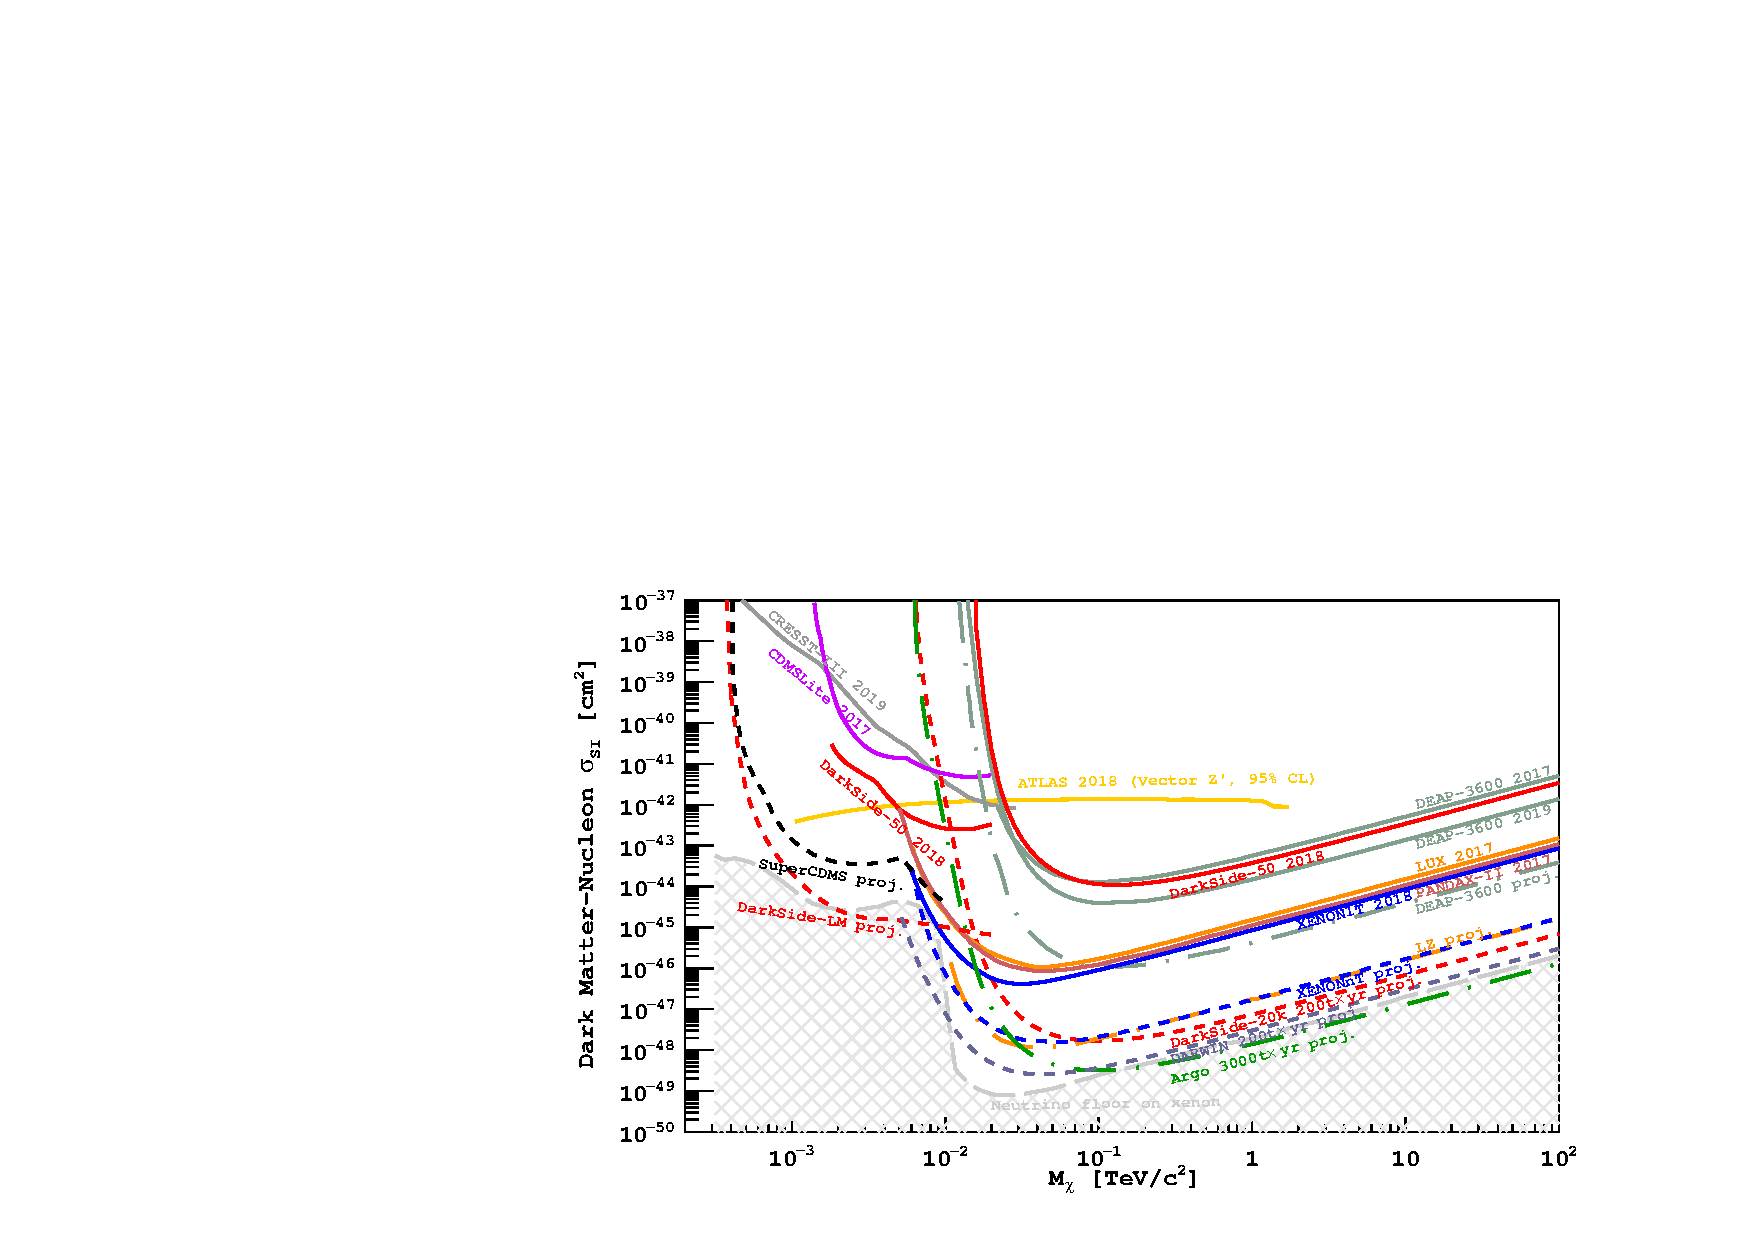
\includegraphics[width=0.9\textwidth]{./Figures/DSklSensitivitySimplified.pdf}
\caption[Current \DM\ limits and sensitivities for future experiments.]
{\SI{90}{\percent} C.L. exclusion limits showing leading results from direct (continuous lines, Ref.~\cite{Angloher:2012kl,Akerib:2017kg,Cui:2017kg,Aprile:2018ct,Agnes:2018ep,Agnes:2018fg}) and accelerator-based dark matter searches (region above the yellow line \cite{TheATLASCollaboration:2018to}) compared with sensitivities of future germanium-, xenon-, and argon-based direct searches (dashed lines, Ref.~\cite{Nelson:2014wy,Kudryavtsev:2015hy,Aprile:2015wv,Boulay:2017tn,Agnese:2017fn} and this work).  The ``neutrino floor'' curve follows the definition of Ref.~\cite{Billard:2014cx}. The 95\% C.L. limit from the ATLAS Experiment is shown for a benchmark model in which Dirac-fermion WIMPs interact with ordinary matter via a vector mediator\cite{Abercrombie:2015to} with coupling strengths to quarks, leptons and WIMPs of 0.25, 0.01, and 1, respectively.
}
\label{fig:DSklSensitivitySimplified}
\end{center}
\end{figure}

Given the potential reach of an argon-based detector, scientists from all of the major groups currently using \LAr\ to search for dark matter, including \ArDM, \DSfs, \DEAP, and \mCLEAN, have joined to form the Global Argon Dark Matter Collaboration (\GADMC) with a goal of building a series of future experiments that maximally exploit the advantages of \LAr\ as a detector target. To this end, the \GADMC\ is developing several novel facilities and techniques. The \Urania\ plant will extract low-radioactivity argon from underground (\UAr) that is naturally depleted in \ce{^39Ar}, the primary intrinsic background in argon extracted from the atmosphere. The \Aria\ cryogenic distillation column will enable the high-throughput purification and active isotopic separation of argon, further reducing \ce{^39Ar} levels and other impurities. Light detection will be done using large-area, cryogenic photodetector modules (\DSkPdms) made with silicon photomultipliers (\SiPMs) optimized for use in \LAr\ and assembled in a custom-built factory. A sealed radio-pure polymethyl methacrylate (\PMMA)  vessel will enclose the TPC, and the entire assembly will operate inside of a membrane cryostat, a technology developed at \CERN\ for \pDUNE, filled with liquified atmospheric argon and operated as a veto detector.

The immediate objective of the \GADMC\ is construction of the \DSks\ two-phase \LAr\ detector, which will operate at the Gran Sasso National Laboratory (\LNGS).  \DSks\ detector will have ultra-low backgrounds and the ability to measure its backgrounds {\it in situ}, resulting in an expected sensitivity to \WIMP-nucleon cross sections of \DSkSensitivityOneGeVUnit\ (\DSkSensitivityTenGeVUnit) for \WIMPMassOneTev\ (\WIMPMassTenTev) \WIMPs\  following a \DSkRunTimePlanned\ run with a total exposure of \DSkExposure.  This projected sensitivity is a factor of~\DSkSensitivityImprovementOneTeV\ better than currently-published results above \WIMPMassOneTev and covers a large fraction of the parameter space currently preferred by supersymmetric models.  During the \DSkExposure\ exposure, \DSkNuInducedBackgroundBare\ \NR\ events are expected from the coherent scattering of atmospheric neutrinos, making \DSks\ the first ever direct dark matter detection experiment to reach this milestone.  The sensitivity would further improve to \DSkExtendedSensitivityOneGeVUnit\ (\DSkExtendedSensitivityTenGeVUnit) for \WIMPMassOneTev\ (\WIMPMassTenTev) WIMPs for a decade-long run with a \DSkExtendedExposure\ exposure, see \reffig{DSklSensitivitySimplified}.  \DSks\ experiment is foreseen to begin operating in 2022 and will either detect \WIMP\ dark matter or exclude a large fraction of favored WIMP parameter space.  As shown in \reffig{NobleDiscoveryComp}, \DSks\ experiment will have discovery sensitivity at the $5\sigma$ level for cross sections much below that probed by the LZ and Xenon-nT experiments and for dark matter masses above the reach of the LHC.
%In case of the observation of a \WIMP\ signal, it would be valuable to have in operation detectors with both \LAr\ and LXe targets such as to cross check each other. 

In parallel to \DSks\ detector, the \GADMC\ collaboration will pursue the development of an approximately \DSlApproxMassScale\ detector specifically optimized for the detection of low-mass dark matter, \DSl\ (\DSls). This detector will be developed at CERN and likely installed and operated at \LNGS. \DSls\ will achieve a lower energy threshold than \DSks\ by triggering on the electroluminescence signal from ionized electrons, thereby adding sensitivity to WIMP masses below \DSlLowMassThreshold\ at the expense of the \PSD\ power afforded by argon prompt scintillation light. Without \PSD, contributors to the \ER\ background in \DSls\ must be reduced beyond the requirements of \DSks\ through careful detector design and material selection.  Based on the world-leading sensitivity for low-mass dark matter achieved with \DSfs\ coupled with the \ce{^39Ar} reduction by distillation available in \Aria\ and the use of a massive \AAr\ veto, this dedicated low-mass detector would have the ability to reach through the so-called ``neutrino floor'' in the low-mass search region, see \reffig{DSklSensitivitySimplified}. While \DSls\ will be developed by the \GADMC, the major funding for this effort will be requested via alternative funding programs.

The ultimate objective of the GADMC is the construction of the \Argo\ detector, which will have a \GADMCFiducialMass\ fiducial mass and will push the experimental sensitivity to the point at which the coherent scattering of atmospheric neutrinos becomes a limiting background. The excellent \ER\ rejection possible in argon will eliminate backgrounds from solar neutrinos, which will extend the sensitivity of \Argo\ beyond that of technologies with more limited \ER\ discrimination. The throughput  of the \Urania\ plant and \Aria\ facility will enable \ArgoTotalMass\ of \UAr\ to be extracted and purified over a period of about \ArgoExtractionPeriod.  At the depth of \SNOLAB, \Argo\ could perform a dark matter search and observe ultra-rare solar neutrino sources (\CNO, \HEP)~\cite{Franco:2016ex}.  While the construction of \Argo\ is not within the scope of this proposal, the implementation of  \DSk\ project will pave the way for the development of \Argo\ towards the end of the next decade. Combined \DSks, \DSls, and \Argo, will completely cover the spin-independent \WIMP\ hypothesis parameter space down to the neutrino floor for WIMP masses from \SI{1}{\GeV\per\square\c} to several hundreds of \si{\TeV\per\square\c}.


%---
\subsubsection{Comparison with Xenon-Based Experiments and the ``Neutrino Floor''}

Next generation dark matter experiments will be sensitive to several sources of neutrinos via $\nu-e$ elastic scattering (\ER) and coherent elastic neutrino scattering (\CEnNS) on nuclei (\NR). Atmospheric and diffuse supernovae neutrinos, which due to their high energies can produce \NRs\ in excess of \SI{20}{\keVr}, will be the dominant \CEnNS\ background contributor for WIMP masses above \DSkHighMassThreshold. Solar neutrinos are the main \CEnNS\ background for dark matter masses below \DSlLowMassThreshold. With  argon's ability to discriminate \ER\ from \NR\ to better than a part in \DEAPPSDRejection, \CEnNS\ represents the only irreducible background for a large exposure argon dark matter search. The neutrino background is exacerbated in liquid xenon detectors, which, due to their limited \ER\ rejection power, accept a non-negligible number of $\nu-e$ elastic scatters as signal. 

When calculating the discovery sensitivity of a large dark matter search experiment, one must fully account for the presence of neutrino-induced backgrounds.  We note that the position of the ``neutrino floor'', initially conceived as indicative of the maximum sensitivity attainable by an experiment in the presence of \CEnNS\ background, is critically dependent on the target, experimental technique, statistical analysis, neutrino flux uncertainty and theoretical cross section uncertainty. We therefore include a detailed accounting of the \CEnNS\ and $\nu-e$ backgrounds in the sensitivity and discovery potential curves shown in \reffig{DSklSensitivitySimplified} and \reffig{NobleDiscoveryComp}. We conservatively estimate a \SI{20}{\percent} uncertainty on the neutrino background for high-mass (\DSkHighMassThreshold) searches with \Argo.  This accounts for a \SI{15}{\percent} uncertainty on the atmospheric neutrino flux at mid-latitude locations, such as \SNOLAB\ or \LNGS, based on the latest data-driven models of cosmic primaries~\cite{Evans:2017hu} as well as models of solar cycle, seasonal, geographic, and geomagnetic dependence of the neutrino flux~\cite{Honda:2011ey,Barr:2006ih}.  Additionally, we account for a \SI{5}{\percent} theoretical uncertainty on the Standard Model interaction cross-section, driven by uncertainties on the nuclear form factor and the expected constraints that the COHERENT collaboration will place on non-Standard Model contributions using a \LAr\ target~\cite{Tayloe:2018jn}, which in turn is driven by their current \SI{10}{\percent} uncertainty on neutrino flux~\cite{Akimov:2017bs} and a \SI{6}{\percent} uncertainty on the \LAr\ response as measured by \SCENE~\cite{Cao:2015ks,Alexander:2013ke} and \ARIS~\cite{Agnes:2018cn}.  Planned improvements of COHERENT, including a sharper characterization of the neutrino flux and a measurement with a \LAr\ target, would further reduce the uncertainty on the neutrino background below \SI{10}{\percent}, strongly benefiting the \DSks, and \Argo\ experiments.

Within this framework, we calculate the 5$\sigma$ discovery potential for \DSks\ and \Argo\ and compare it with that of the near-future \LXe\ experiment LZ~\cite{Dobson:2018us}.  As seen from \reffig{NobleDiscoveryComp}, \DSks\ has significantly greater discovery potential than that of LZ.


%The \CEnNS\ process, recently observed by the COHERENT experiment~\cite{Akimov:2017bs}, appears in line with the Standard Model prediction~\cite{Hasert:1973dm,Hasert:1973hj,Hasert:1974eh,Freedman:1974bd,Drukier:1984fo}.


\begin{figure}
\begin{center}
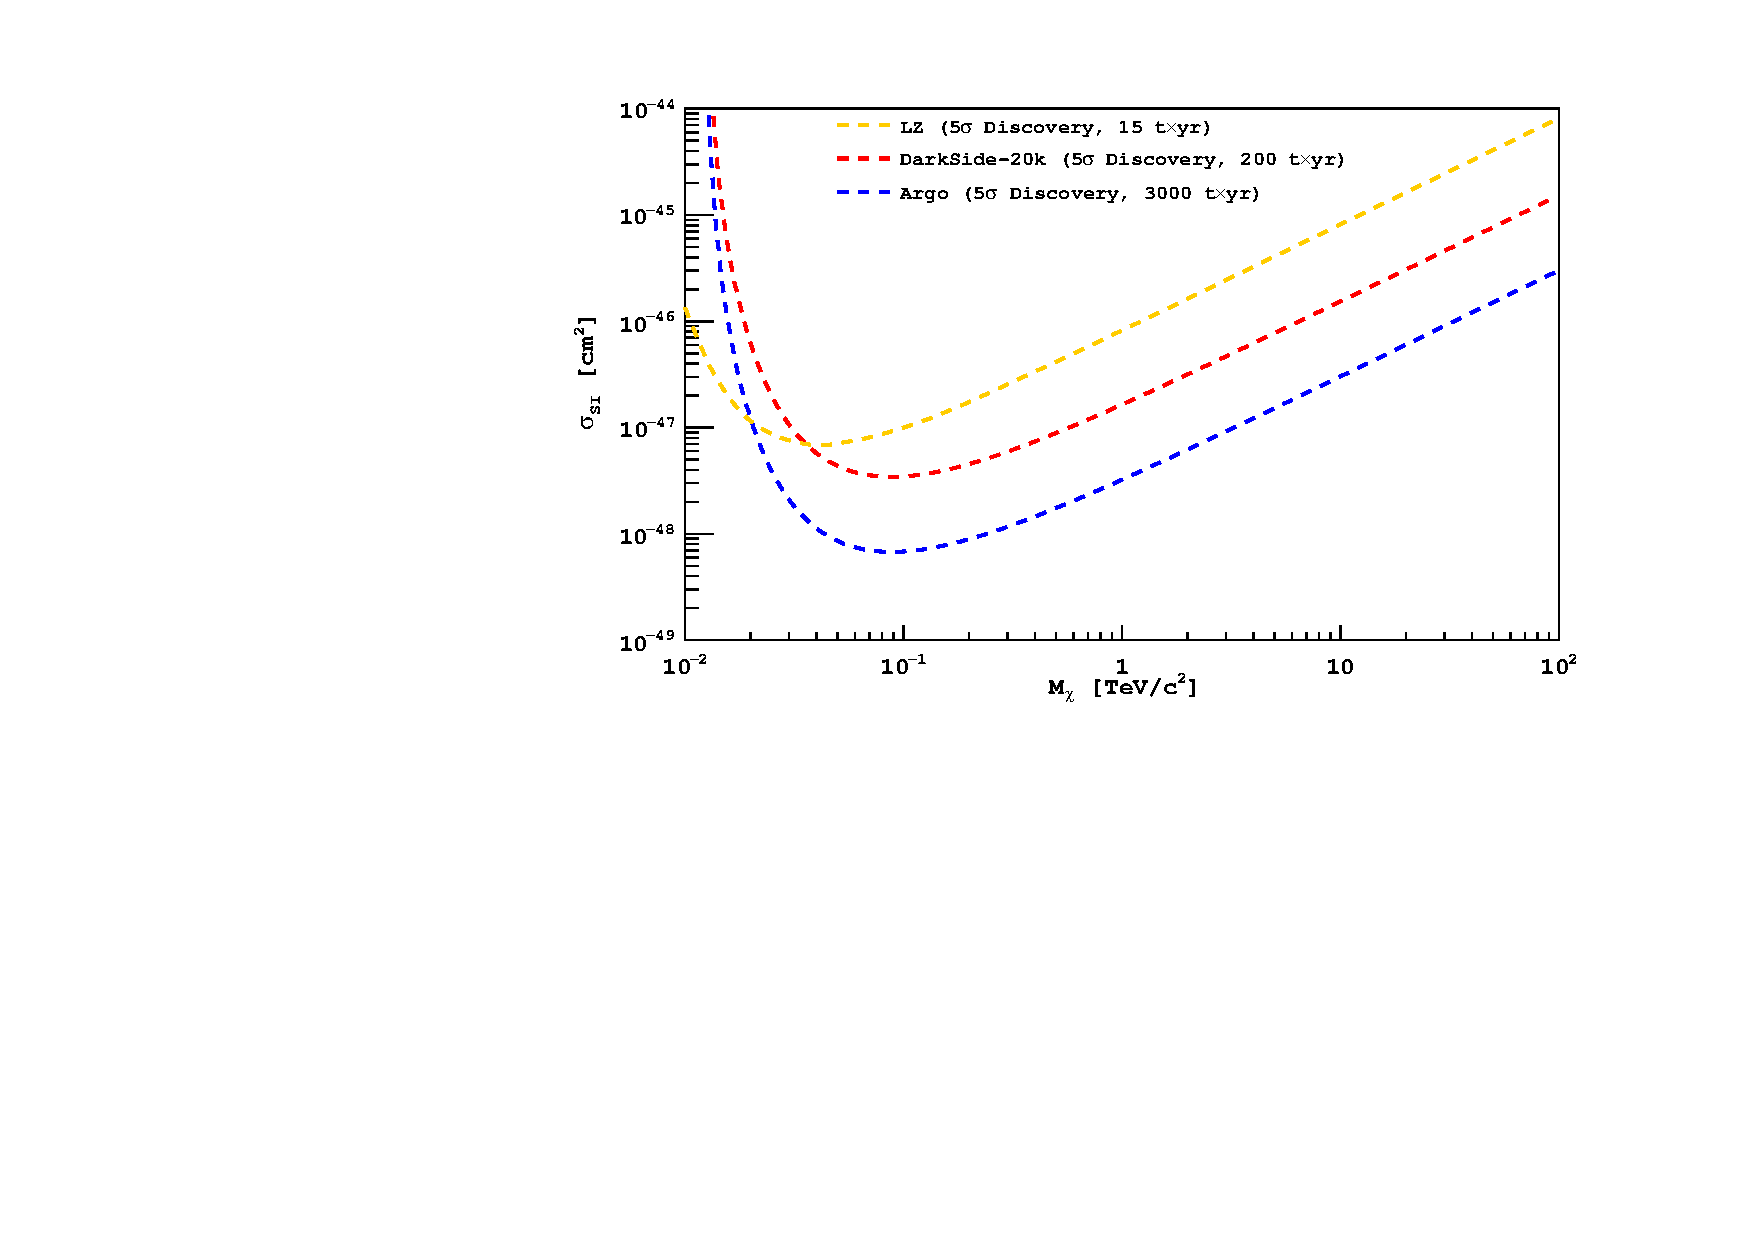
\includegraphics[width=0.7\textwidth]{./Figures/NobleDiscoveryComp.pdf}
\caption{5$\sigma$ discovery potential of the leading future noble liquid dark matter searches.  %See \reftab{NobleExpComp} for details and sources.
}
\label{fig:NobleDiscoveryComp}
\end{center}
\end{figure}

%\begin{table}[t!]
%\begin{tabular}{lcccc}
%\hline\hline
%Experiment	&Target		&Threshold [\si{keVr}]
%										&Exposure [\si{\tonne\year}]
%																&Source\\
%\hline
%LZ			&\LXe		&\num{4}		&\num{15}				&\cite{Dobson:2018us}\\
%\DSk		&\LAr		&\num{30}		&\num{200}				&This work\\
%\hline
%DARWIN		&\LXe		&\num{7}		&\num{200}				&\cite{Aalbers:2016ex}\\
%\Argo		&\LAr		&\num{30}		&\num{3000}				&This work\\
%\hline\hline
%\end{tabular}
%\caption{Comparison of characteristics and expected performance of future \LXe\ and liquid argon \LAr\ direct detection dark matter experiments.}
%\label{tab:NobleExpComp}
%\end{table}



%---
\subsubsection{New Technologies}
\label{sec:technologies}

The following technologies are key to the success of \DSk\ project and the long term scientific goals of the \GADMC. Their development will also have potentially wide-reaching effects within the physics community.

{\bf Low-radioactivity underground argon with Urania~\cite{Aalseth:2018gq}:} 
The \DSfs\ experiment established that \UAr\ is depleted of \ce{^39Ar} by a factor of approximately 1400, a sufficiently low rate to be deployed in a detector the size of \DSks. However, constructing \DSks\ will require that large amounts of \UAr\ be procured in a timely fashion. This will be accomplished by Urania, an argon extraction and purification plant capable of extracting \UraniaUArRate\ of \UAr.  The Urania plant is fully funded by the INFN and will be built by a contracted vendor following specifications established by the Urania Project team. The tender process for the plant's final design, construction, and shipment to the installation site in Cortez, Colorado, is underway and will conclude by the of end of July 2019 with the selection of a contractor.  The preparation of the extraction site, as well as the installation and commissioning of the plant, falls under the responsibility of the U.S. \NSF-supported groups.  The Urania \UAr\ extraction plant is projected to collect approximately \UraniaTotalDSkProduction\ of argon for use in \DSks\ detector by 2022 and could continue to produce underground argon for \Argo\ and other interested particle physics experiments that require \UAr\ to achieve their scientific objectives.  

{\bf Purification and active depletion with Aria~\cite{Aalseth:2018gq}:}
The \Aria\ plant is a \SI{350}{\m} tall cryogenic distillation column that was designed to explore the possibility of chemically separating argon isotopes.  The construction of \Aria\ is fully supported by \INFN\ and the Regione Autonoma della Sardegna. 
 %Fabrication of the individual modules that make up the first of two \SI{350}{\m} columns, \SeruciOne, is complete and their installation in a vertical mine shaft in Sardegna, Italy, will begin in June 2019.  A \AriaNuraxiHeight\ surface prototype, \SeruciZero, has recently been completed and will start operations in June 2019.  The \SeruciOne\ plant is estimated to be able to process \UAr\ at a rate of \AriaSeruciOneRate, obtaining a \ce{^39Ar} depletion factor of \AriaDepletionPerPass\ per pass and enabling further suppression of \ce{^39Ar} by two or three orders of magnitude. This will play a crucial role in the science reach of \DSls.

{\bf SiPM-based cryogenic photosensors~\cite{Aalseth:2018gq,DIncecco:2018hy,DIncecco:2018fx}:}
The development of low-background, large-area, cryogenic silicon photomultiplier (SiPM) detectors capable of replacing conventional photomultiplier tubes is critically important for achieving the desired sensitivity of \DSks\ and other large-scale \LAr-based experiments, including DUNE, and LXe-based detectors, such as \nEXO~\cite{Ostrovskiy:2015jl} and NEXT~\cite{Cebrian:2017dy,GomezCadenas:2016cm,Cebrian:2015du}.  The \DSks\ photodetector modules will be assembled at the Nuova Officina Assergi (\NOA), a dedicated cleanroom packaging facility that will have future utility for any experiment needing large volume silicon detector production.

% \SiPMs\ have a number of performance advantages over traditional PMTs, including higher photo-detection efficiency and much better single-photon resolution, all while operating at much a lower bias voltage.  \SiPMs\ can also be efficiently integrated into tiles that cover large areas and feature better radiopurity, by up to an order of magnitude, compared to traditional photomultiplier tubes (\PMTs). 

{\bf \pDUNE\ liquid argon cryostat~\cite{Abi:2017wp,Acciarri:2016wz}:}
\DSks\ detector will operate within a membrane cryostat filled with liquefied atmospheric argon, a technology initially developed at \CERN\ for \pDUNE. Eliminating the organic liquid scintillator veto used in \DSfs\ for the \AAr\ veto has several advantages. With the the \DSks\ \LArTPC\ directly immersed in \AAr, the massive stainless steel vacuum cryostat necessary for \DSfs, and its correspondingly large contribution of background events, can be replaced with a transparent, radio-pure \PMMA\ vessel. Photodetector modules can then be mounted outside of the \PMMA\ vessel, reducing their contribution to the background rate and simplifying their assembly strategy. The \pDUNE\ cryostat has the added advantage that it is scalable, making it a technology appropriate for \Argo.

{\bf Sealed acrylic TPC~\cite{Boulay:2012er,Nantais:2013jp,Amaudruz:2018gr}:}
The \DEAP\ collaboration has extensive experience developing large, radio-pure sealed \PMMA\ vessels. This technology will be used to build the vessel for the \DSks\ \LArTPC, eliminating the need for some of the most problematic radiogenic neutron contributors in \DSfs, already mentioned stainless steel cryostat as well as the \PTFE\ reflector. The \PMMA\ vessel will also reduce the complexity of the \TPC\ assembly.

%---
\subsection{Research Community Benefits}
%{Description of the infrastructure in the context of, for example, the project's potential benefit to the broader I.S. research community (e.g. access to infrastructure, new research resources, data products, etc.).  Describe how the proposed infrastructure responds to identified high-priority needs of a research community.}

\subsubsection{Relation to NSF's 10 Big Ideas}

{\bf Growing Convergence Research:}
The \GADMC\ was built to connect experts from a variety of disciplines to answer one of science's biggest questions: what is dark matter? The interdisciplinary collaboration consists of physicists from various sub-disciplines, engineers from a wide-range of specialties, chemists, and computer and data scientists.  The \GADMC\ has also built strong partnerships with a number of companies and foreign regional governments, which are either investing in the effort with funding or in-kind contributions. These connections bridge the gap between disparate professions and research groups operating at locations all over the world. This environment gives our students and young scientists broad exposure to an array of fields, professions, and cultures, helping them become experienced, versatile, and technically skilled researchers.

{\bf Harnessing the Data Revolution:}
As in many of today's large-scale particle physics experiments, many petabytes of physics, calibration, and monte carlo simulation data will be collected, analyzed, and stored over the course of the 5 year \DSks\ operation. The collaboration is exploring new methods for storing and processing this data, including the use of machine learning algorithms for reconstruction, smart batch-data processing, and high-level physics analyses.  The implementation of the \DSks\ detector and its operation will expose a new generation of young researchers to big-data analysis. 
%In particular, the \DSks\ data, due to the large number of \ER\ background events expected,  will have a massive class-imbalance. This creates an opportunity for to test new machine learning algorithms along with traditional analysis methods and for the comparison of their respective effectiveness.  This is a common problem in many areas of interest for the broader information technology community, and \DSks\ will provide one more opportunity for the development in the basic research environments of solutions that can be adapted to other real-world problems.

{\bf Mid-scale Research Infrastructure:}
The \DSks\ experiment falls under the definition of an NSF Mid-scale Research Infrastructure as outlined in \NSF's ``Bridging the Gap: Building a Sustained Approach to Mid-scale Research Infrastructure and Cyberinfrastructure at \NSF.''  The 2015 \DSk\ proposal was approved by \INFN\ and \NSF\ in 2017 following a detailed review of the first version of the \DSk\ Project Execution Plan.  \LNGS\ also approved the experiment for installation in 2017.  In 2018, \DSk\ project was approved as Recognized Experiment 37 (RE-37) at \CERN.  The \DSks\ detector facility will be one of the most sensitive detectors in the world searching for \WIMPs, enabling unique opportunities to train the next generation of the scientific workforce.

{\bf NSF INCLUDES:}
The U.S. \DSk\ effort will leverage the involvement of Fort Lewis College in Durango, Colorado, to increase inclusion of underrepresented groups.  Since its founding in 1911, Fort Lewis College has demonstrated a unique commitment to the education of the local Native American population, in compliance with the deed that transferred the property of the former Fort Lewis from the Federal Government to the State of Colorado under condition that the land would be used for an educational institution, ``to be maintained as an institution of learning to which Indian students will be admitted free of tuition and on an equality with white students'' in perpetuity (Act of 61st Congress, 1911).  With this proposal, we request support to re-establish the Princeton-Gran Sasso Summer School for Physics. In the US, we will target high-school seniors and college freshman students from the Cortez-Durango area, offering them a period of study at Princeton, followed by a research period spent either at the Colorado Urania facility, the Aria facility in Sardinia, at LNGS, or at CERN.  This will expose them to otherwise unavailable on-site training and provide them with a network for pursuing job opportunities in the future, both through the project scientists and the companies partnered with the project.  The participation of students from the Cortez-Durango area may be complemented with that of high-school students from the Italian regions of the argon trail, {\it i.e.} Sardegna and Abruzzo. Funds for the participation of the Italian students will be independently sought from Italian government sources.

{\bf Windows on the Universe:}
Recently, the Supernova Early Warning System (SNEWS) team submitted a proposal to the NSF Windows on the Universe solicitation for an upgrade to their system that enhance their capabilities.  \DSks\ was included in that proposal as a future partnering experiment that will work with the SNEWS network to detect galactic supernova neutrino bursts and provide an early warning of the incoming photon and gravitational wave signals.  The \DSks\ detector will have the unique ability to measure the supernova neutrinos in a flavor-blind way, meaning it will be able to constrain the total flux and the mean energy of the neutrinos over the duration of the burst.  This measurement, coupled with the neutrino measurements of other experiments and the photon and gravitational wave measurements, will provide a multi-messenger probe of a galactic supernova capable of differentiating between explosion mechanisms, characterizing neutron stars, studying black hole formation, answering general questions in particle physics and astrophysics, and providing new insight into neutrino oscillations.


%---
\subsubsection{Community Recommendations}

In the U.S., the 2014 report of the Particle Physics Project Prioritization Panel (P5) ``Building for Discovery - Strategic Plan for U.S. Particle Physics in the Global Context''~\cite{ParticlePhysicsProjectPrioritizationPanel:2014td} acknowledges:

{\it Technologies with major U.S. participation include: two-phase xenon; single- and two-phase argon; cryogenic germanium and silicon; bubble chambers; sodium iodide crystals; and directional time-projection chambers. The preeminent challenge in this field is the elimination of backgrounds, with approaches including the use of low background materials, self-shielding, particle identification, and astrophysical rate modulation.}

It then states:

{\it The experimental challenge of discovery and characterization of dark matter interactions with ordinary matter requires a multi-generational suite of progressively more sensitive and ambitious direct detection experiments.  This is a highly competitive, rapidly evolving field with excellent potential for discovery.  The second-generation direct detection experiments are ready to be designed and built, and should include the search for axions, and the search for low-mass ($<$10 GeV) and high-mass WIMPs.  Several experiments are needed using multiple target materials to search the available spin-independent and spin-dependent parameter space.  This suite of experiments should have substantial cross-section reach, as well as the ability to confirm or refute current anomalous results.  Investment at a level substantially larger than that called for in the 2012 joint agency announcement of opportunity will be required for a program of this breadth.}

And recommends:

{\it Recommendation 19: Proceed immediately with a broad second-generation (G2) dark matter direct detection program with capabilities described in the text.  Invest in this program at a level significantly above that called for in the 2012 joint agency announcement of opportunity.}

It then states:

{\it The results of G2 direct detection experiments and other contemporaneous dark matter searches will guide the technology and design of third-generation experiments.  As the scale of these experiments grows to increase sensitivity, the experimental challenge of direct detection will still require complementary experimental techniques, and international cooperation will be warranted.  The U.S. should host at least one of the third-generation experiments in this complementary global suite.}

And also recommends:

{\it Recommendation 20: Support one or more third-generation (G3) direct detection experiments, guided by the results of the preceding searches.  Seek a globally complementary program and increased international partnership in G3 experiments.}

In Europe, the ``European Astroparticle Physics Strategy 2017-2026''~\cite{AstroparticlePhysicsEuropeanConsortium:2017wy} authored by the ``Astroparticle Physics European Consortium'' (APPEC) identifies the following as one of the key questions in Astroparticle Physics:

{\it ``The Dark Universe: What is the nature of Dark Matter and Dark Energy?''}

In addition, it states:

{\it Medium-scale Dark Matter and neutrino experiments: APPEC considers as its core assets the diverse, often ultra-precise and invariably ingenious suite of medium-scale laboratory experiments targeted at the discovery of extremely rare processes.  These include experiments to detect the scattering of Dark Matter particles and neutrinoless double-beta decay, and direct measurement of neutrino mass using single-beta decay.  Collectively, these searches must be pursued to the level of discovery, unless prevented by an irreducible background or an unrealistically high demand for capital investment.}

It then adds:

{\it Elucidating the nature of Dark Matter is a key priority at the leading tip of astroparticle physics.  Among the plethora of subatomic particles proposed to explain the Dark Matter content of our Universe, one category stands out: the Weakly Interacting Massive Particle (WIMP).  WIMPs arise naturally, for instance, in supersymmetric extensions of the Standard Model of particle physics. Many experiments located in deep-underground laboratories are searching for WIMP interactions.  For masses in excess of a few GeV, the best sensitivity to WIMPs is reached with detectors that use ultra-pure liquid noble-gas targets; such detectors include XENON1T (using 3.5 tons of xenon) and DEAP (using 3.6 tons of argon), which both started operating in 2016.  Their sensitivity can be further enhanced by increasing the target mass. A suite of smaller-scale experiments is exploring, in particular, low-mass WIMPs and other Dark Matter hypotheses such as those based on dark photons and axions.}

It continues:

{\it The highest sensitivity for WIMPs in a mass range of around 5 GeV to 10 TeV is reached by experiments using, as a target, liquid xenon (notable examples include LUX in the US, PandaX in China and XENON100 in Italy) and liquid argon (e.g. DEAP in Canada, DarkSide-50 in Italy, pioneering the use of argon depleted in argon-39, and ArDM in Spain).  A ton-scale xenon detector, XENON1T, is being commissioned and, after two years of continuous operation, can access cross- sections as low as 10$^{-47}$ per centimetre squared.  For the near future, multi-ton-scale liquefied noble-gas detectors with strong European participation are already at an advanced planning stage: namely, XENONnT (8 tons of xenon), LZ (7 tons of xenon) and DarkSide-20k (20 tons of argon).  For lower-mass WIMPs (below 6-7 GeV), the best performance is achieved using a combination of light and heat signals or ionisation and heat signals in cryogenic detectors cooled down almost to absolute zero: for example, CRESST (at LNGS in Italy) combines light and heat signals, while EDELWEISS (at LSM in France) combines ionisation and heat signals.  In the U.S. and Canada, SuperCDMS and DAMIC are also pursuing low-mass dark matter.}

And it concludes:

{\it APPEC encourages the continuation of a diverse and vibrant programme (including experiments as well as detector R\&D) searching for WIMPs and non-WIMP Dark Matter. With its global partners, APPEC aims to converge around 2019 on a strategy aimed at realising worldwide at least one `ultimate' Dark Matter detector based on xenon (in the order of 50 tons) and one based on argon (in the order of 300 tons), as advocated respectively by DARWIN and Argo.}


%---
\subsubsection{\DSk: The High-Mass Search Program}
\label{sec:DSk}

\DSks\ will be located in Hall-C of the Gran Sasso National Laboratory (\LNGS) in Italy. It consists of two nested detectors housed within a \pDUNE-style membrane cryostat~\cite{Abi:2017wp,Acciarri:2016wz}.  

The inner detector is a dual-phase argon time projection chamber (\LArTPC) contained within an acrylic vessel made from ultra-pure poly(methyl methacrylate) (\PMMA) and filled with \UAr.  The central active volume of the TPC is defined by eight vertical reflector panels and the top and bottom windows of the acrylic vessel. Instead of the traditional copper field cage rings and Indium-Tin-Oxyde (\ITO) cathode and anode, \DSks\ will use poly(3,4-ethylenedioxythiophene) polystyrene sulfonate (also known as \PEDOT\ and commercialized under the name \Clevios~\cite{HeraeusDeutschlandGmbHandCOKg:2019wt}). All the TPC surfaces in contact with the active argon volume will be coated with \TPB\ wavelength shifter to convert \LAr\ scintillation light to a wavelength detectable by \SiPMs.  \DSkTilesNumber\ \SiPM-based \DSkPdm\ arrays will view the argon volume through the top and bottom windows of the acrylic vessel. The height of the \TPC\ is \DSkTPCHeight. With this design, the total mass of LAr in the active volume is \DSkActiveMass.

The outer veto detector is made of a passive \ce{Gd}-loaded \PMMA\ shell, which surrounds the inner detector, sandwiched between two active \AAr\ layers.  The \ce{Gd}-loaded \PMMA\ shell moderates neutrons emitted from the \LAr\ \TPC\ until they capture on \ce{Gd}, resulting in the emission of multiple \grs.  The \grs\ interact in the \AAr\ layers and cause scintillation light that is detected by photodetectors, thereby providing an efficient veto of radiogenic neutrons that could result in a \NR\ in the TPC.  The \pDUNE-like cryostat will be surrounded by layers of plastic to moderate cosmogenic and radiogenic neutrons from the rocks surrounding Hall~C.

\reffig{DSk3D} shows a 3D schematic of the \DSks\ detector. \DSks\ is designed to operate with zero backgrounds, i.e., all sources of instrumental background reduced to \BackgroundFreeRequirement\ over a \DSkExposure\ exposure.  The only remaining background will be that coming from the coherent scattering of neutrinos from argon nuclei. While coherent neutrino scattering is a background for the WIMP search, this sensitivity is a feature that enables \DSks\ to detect a supernova neutrino burst coming from anywhere in the Milky Way Galaxy and, for a majority of the galaxy, clearly identify the neutronization burst. \DSks\ would perform a flavor-blind measurement of the total neutrino flux and average energy, setting an overall normalization that is not affected by neutrino oscillations. When combined with a flavor-specific measurement from a detector like Super-Kamiokande or DUNE, this observation could have sensitivity to the neutrino mass hierarchy.  

 
\begin{figure}[t!]
\begin{center}
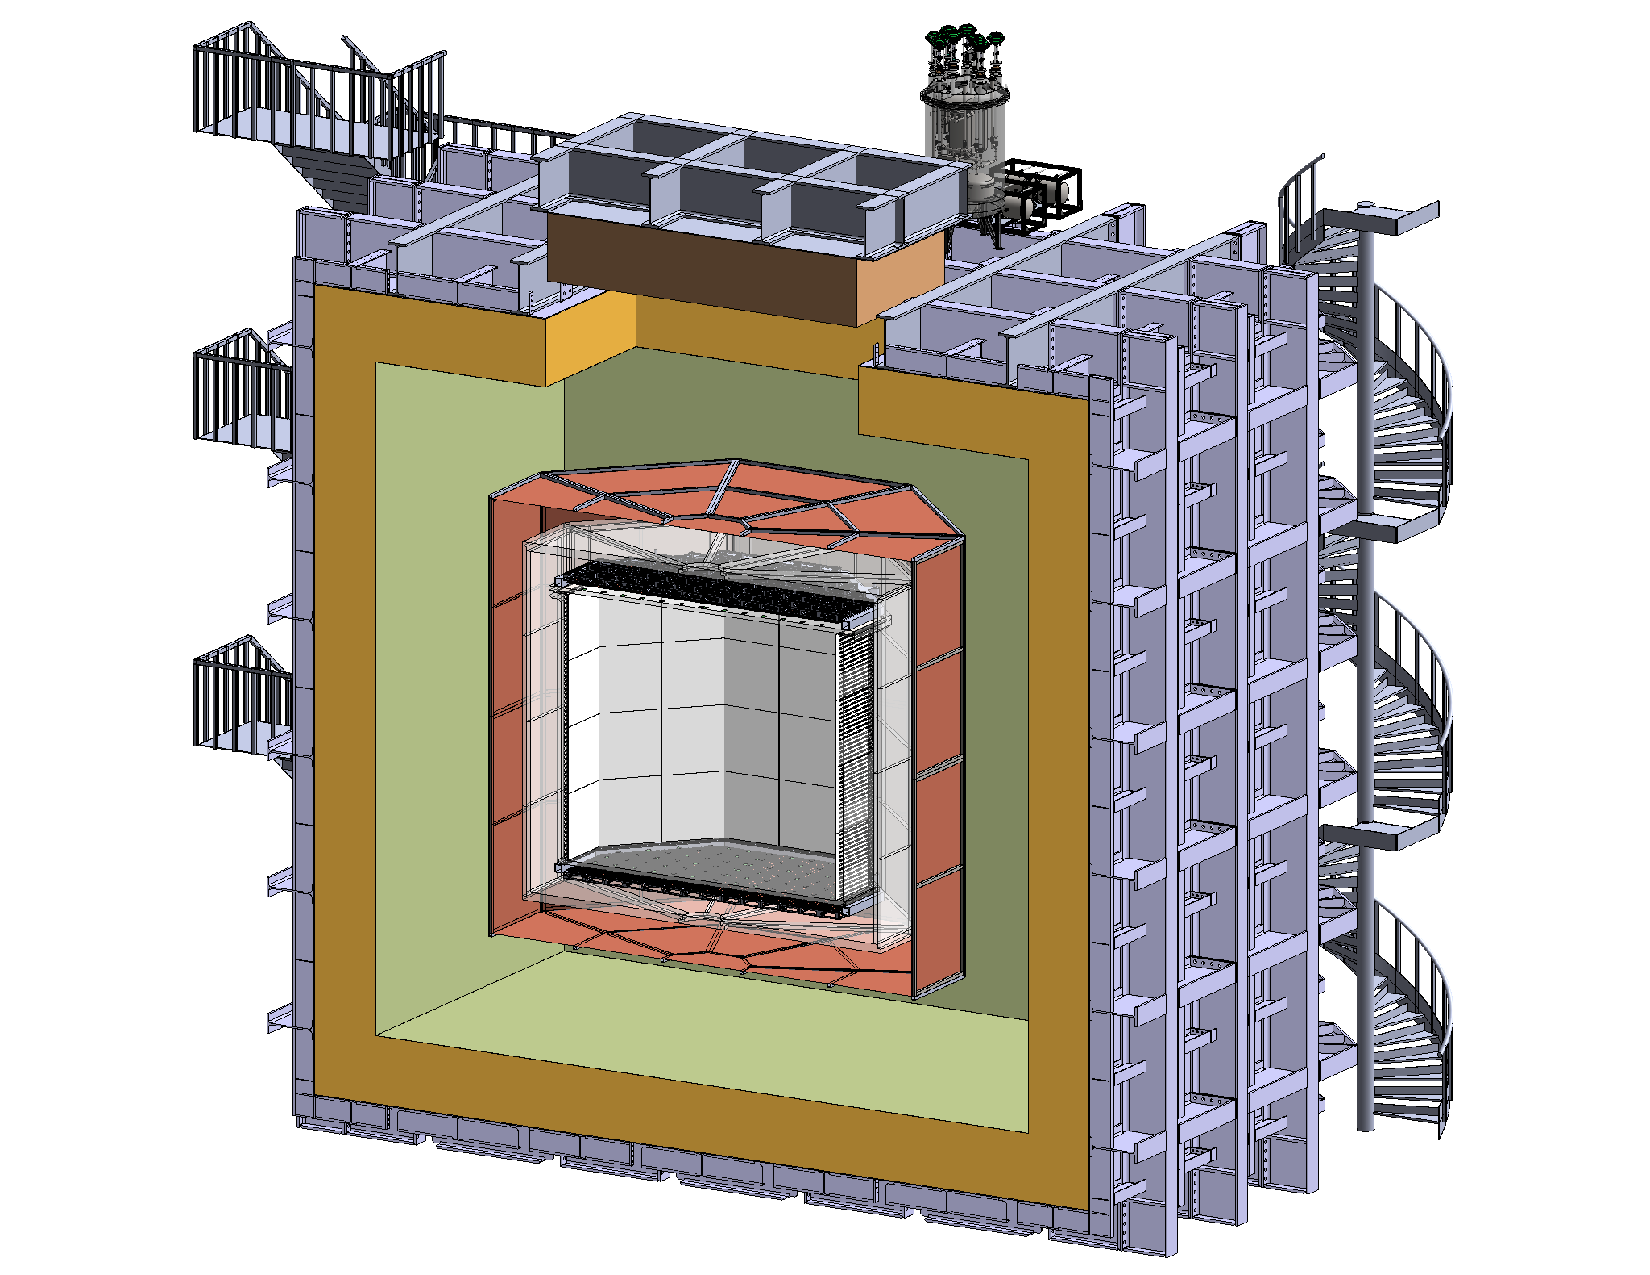
\includegraphics[width=0.45\textwidth]{Figures/DSk3D.pdf}
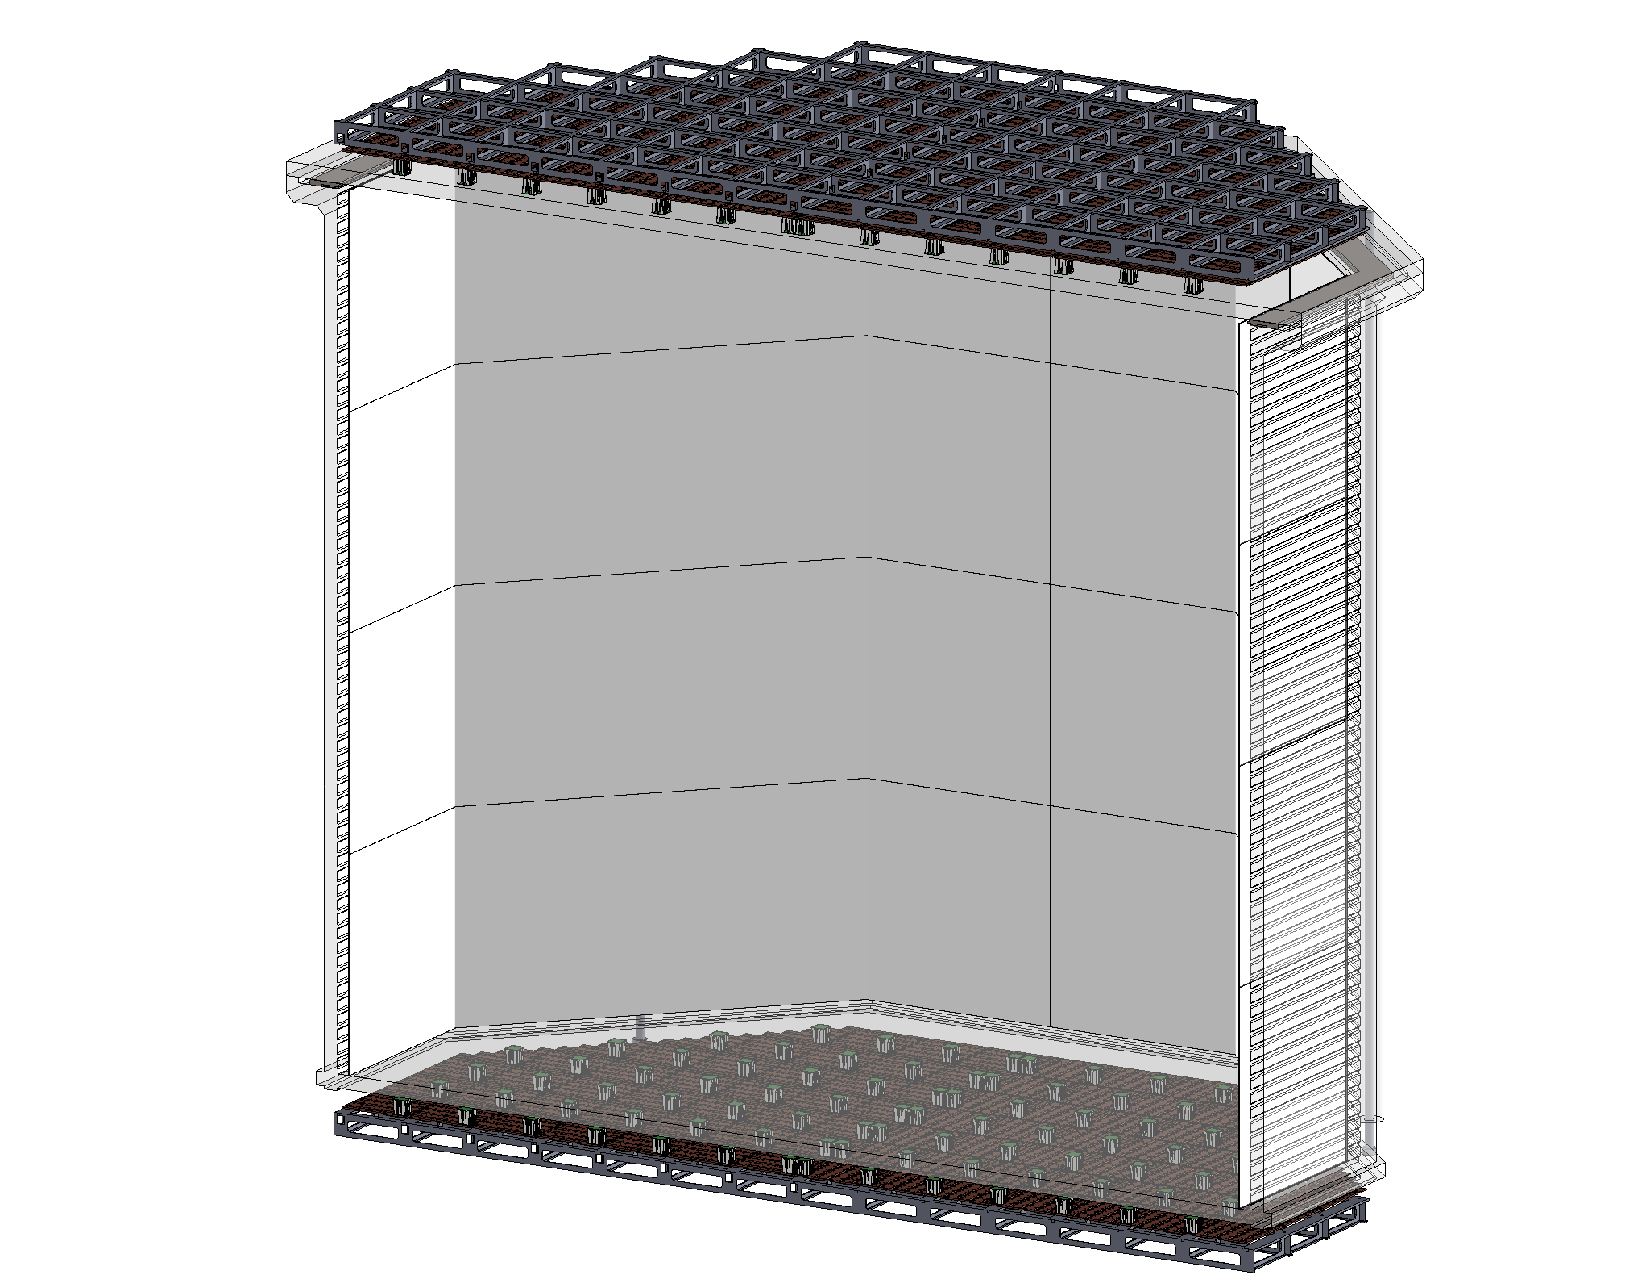
\includegraphics[width=0.45\textwidth]{Figures/DSkTPC.pdf}
\end{center}
\caption{The \DSks\ detector. {\bf Left}: The \PMMA\ \TPC\ filled with \UAr, surrounded by the veto detector made of a \ce{Gd}-loaded \PMMA\ shell sandwiched between two \AAr\ active layers, all contained within a membrane cryostat. The outer active argon layer is optically separated from the \AAr\ by a membrane, whose characteristics are yet to be defined. {\bf Right}: A detailed view of the \TPC.}
\label{fig:DSk3D}
\end{figure}

This proposal requests funds for the U.S. contribution to the construction and commissioning of the \DSks\ detector at \LNGS\ and the Urania \UAr\ extraction facility, which will produce \UAr\ for the inner detector. There are six major areas that the U.S. NSF-supported groups will contribute to: the Urania plant installation and commissioning, photoelectronics development and fabrication, cryogenics and gas handling system design and fabrication, inner detector design and component fabrication, and development of calibrations sources and systems.  The responsibility of each NSF-supported group is outlined in the accompanying statements of work and other supplemental materials. These are critical components of the \DSk\ project that require the technical expertise and resources of the U.S. groups.


%---
\subsubsection{\DSl: The Low-Mass Search Program}
\label{sec:DSl}

While the \DSls\ experiment is outside the scope of this proposal, the implementation of \DSk\ project will have direct impacts on the technological advancements required to enable \DSls\ and the goal of reaching the neutrino floor for WIMP masses between \SI{1}{\GeV\per\c\squared} and \SI{10}{\GeV\per\c\squared}. Among these are the development of low-background \DSkPdms~\cite{DIncecco:2018fx,DIncecco:2018hy} and the construction of the \Aria\ cryogenic distillation column, which will completely remove \ce{^85Kr} and reduce \ce{^39Ar} levels to the level of \SI{1}{\micro\becquerel\per\kg}


% \DSls\ will initially be constructed at \CERN\ to support tests of the \DSks\ elements, and in particular the \DSkPdms~\cite{DIncecco:2018fx,DIncecco:2018hy}.  Thanks to the use of the low-background \SiPM-based \DSkPdms, a low-background cryostat, and an ultra-low background argon target purified by the \Aria\ cryogenic distillation column, \DSls\ will perform a competitive and compelling exploration of the low-mass discovery region, reaching into the neutrino floor.
%
%The world-leading low-mass results of \DSfs\ were enabled by the use of the ionization signal from very low energy events.  The analysis threshold was  \DSfLowMassThresholdEe\ (\DSfLowMassThresholdNr), corresponding to \DSfLowMassThresholdE\ extracted from the liquid target, with each electron producing in average, by electroluminescence, \DSfLowMassThresholdPE.  The residual background above \SI{7}{\el} (\SI{1.2}{\keVr}) in \DSfs\ was completely characterized and accounted for by known sources: the dominant components were the residual target contaminations in \ce{^39Ar} and \ce{^85Kr} and radioactive contamination of the PMTs.
%
%The \DSls\ \TPC\ will be a scaled-down version of that of \DSks, can be operated in a low-radioactivity copper container, and within a \AAr\ active veto.  Thanks to the \Aria\ cryogenic distillation column, we are able to project the complete removal of \ce{^85Kr} and the reduction of \ce{^39Ar}, for small, \si{tonne}-size batches, to the level of \SI{1}{\micro\becquerel\per\kg}.  The limiting low-energy background from \DSkPdms\ can be reduced by the use of ultra-pure light guides and by planned abatements of the radioactivity of the \DSkPdms\ components.
%
%Detailed studies show the background limiting the analysis threshold to \DSfLowMassThresholdE\ in \DSfs\ is related to the impurity and radioactivity levels in the active volume.  Thus, we plan on a strong reduction of both impurity and radioactivity levels by using novel noise and contamination techniques~\cite{Sorensen:2017wo,Sorensen:2017vb,Sorensen:2018jh}, advanced paths for purification of the region at the boundary between the two phases, enhancement of the overall purification rate of the bulk liquid, and use of advanced fiducialization techniques, to achieve a very strong reduction of background and to lower the analysis threshold to \SI{2}{\el}, opening the way to reach the sensitivity shown in \reffig{DSklSensitivitySimplified}.
%
%An improved knowledge of the ionization distribution of nuclear recoils is needed to reduce the uncertainties in the expected signal yield above the analysis threshold and thus improve the sensitivity at the lowest masses.  As part of the \GADMC\ program, we plan to study low energy nuclear recoils by performing direct measurements of scintillation and ionization yield using a neutron-beam in the \ReD\ experiment, and we  plan to perform dedicated studies in the energy range of interest for low mass DM detection (\SI{<1}{\keVr}), with the specific goal of the first direct measurement of the ionization yield in liquid argon at such low energies and, possibly, of establishing a realistic and detailed model for fluctuations of ionization of nuclear recoils.


%---
\subsubsection{Argo}
\label{sec:Argo}

The \GADMC\ is planning a phased approach towards reaching the neutrino floor for high-mass \WIMPs\ ($>$\SI{10}{\GeV\per\c\squared}).  \DSks, the objective of this proposal, with its planned \DSkExtendedExposure\ exposure will reach a sensitivity approximately \DSkImprovementOverDEAP\ times beyond that of \DEAP, which has a design exposure of \DEAPExposure.  After \DSk\ project, the collaboration plans to construct the \Argo\ detector for an ultimate dark matter search with an exposure of \ArgoExtendedExposure, a factor of \ArgoImprovementOverDSk\ improvment.  Support for \Argo\ is not requested as part of this proposal, but work on \DSk\ project will enable this future program.  We anticipate a detector with a fiducial mass of approximately \ArgoFiducialMass, with the experiment starting around \ArgoStartDate. In addition to dark matter detection, such a large detector would also have excellent sensitivity to a neutrino burst associated with a galactic supernova.  If located at \SNOLAB\ or at similar depth, \Argo\ will also have the potential to detect \CNO\ neutrinos for the first time and solve the Solar Metallicity Problem~\cite{Franco:2016ex}. 